\documentclass[a4paper, 12pt, titlepage]{report}
\usepackage{minted}
\usepackage[dvipsnames]{xcolor}
\colorlet{LightApricot}{Orchid!20}
\usepackage{graphicx}
\usepackage{fullpage}
\usepackage{float}
\usepackage{hyperref}
%\usepackage{longtable}
%\usepackage{amsmath}
%\usepackage[normalem]{ulem}
\usepackage{booktabs}
\usepackage{dirtree}
\usepackage{hologo}
\usepackage{csquotes}
\usepackage{tikz}
\usetikzlibrary{shapes.geometric, arrows}

%\usepackage{array}
%\usepackage{tikz}
%\usepackage{parskip}
%\newcommand{\tabitem}{~~\llap{\textbullet}~~}
\setlength{\tabcolsep}{18pt}
\renewcommand{\arraystretch}{1.5}
\renewcommand{\chaptername}{Section}
\hypersetup{
    colorlinks=true,
    linkcolor=blue,
    filecolor=magenta,
    urlcolor=RoyalBlue,
}
\begin{document}
\tikzstyle{startstop} = [rectangle, rounded corners, minimum width=3cm, minimum height=1cm,text centered, draw=black, fill=red!30]
\tikzstyle{io} = [trapezium, trapezium left angle=70, trapezium right angle=110, minimum width=3cm, minimum height=1cm, text centered, draw=black, fill=blue!30]
\tikzstyle{process} = [rectangle, minimum width=3cm, minimum height=1cm, text centered, text width=4cm, draw=black, fill=orange!30]
\tikzstyle{decision} = [diamond, minimum width=3cm, minimum height=1cm, text centered, draw=black, fill=green!30]
\tikzstyle{arrow} = [thick,->,>=stealth]
\linespread{1.25}
\author{Affaan Muhammad - 33016763\\Joshua Esterhuizen - 30285976}
\title{ITRI615 - Computer Security\\Project Documentation}
\date{}
\maketitle
\tableofcontents{}
\chapter{Cryptographic Schemes and Background}
\section{Vigenère Cipher}
This cipher was first described by Giovan Bellaso in 1553 but later misattributed to Blaise de Vigenère, hence its name. This cipher works by making use of a series of interwoven Caesar ciphers - which when joined create a Vigenère Table - based on the letters of a given keyword. As such, it is a polyalphabetic substitution cipher. It was still "indecipherable" almost three centuries after its development.
\subsection{Our Implementation}
Our Vigenère algorithm implementation makes use of:
\begin{itemize}
\item a function to extend the user given key to match the message or file content's length.
\end{itemize}
\subsection{The Algorithm Itself}
Our Vigenère algorithm implementation works using calculations involving the ASCII values of the letters, and byte characters in a file's case, to apply the same effect of a Vigenère Table. The encryption adds these values within modulo26 for text (also adding 65 as discussed below) and modulo256 for files while the decryption subtracts these values. When it comes to the text "mode" of this algorithm, we have included a check to ensure that all characters that have the cipher applied are indeed letters. This is done by:
\begin{itemize}
\item Before the algorithm takes place, we apply the ".upper()" to the text string to keep all characters as capital letters,
\item Setting an if statement that riggers if the ASCII value of a character is not within the capital letter values,
\item Immediately append to the array that will be returned.
\end{itemize}
We could also do the same process above but with lowercase letters with ".lower()" if we so chose.
\subsection{The Key Extender}
As with the "normal" and our implementation of the Vigenère cipher algorithm, the user provided key mmust be repeated across the length of the message. This function does nothing if the key provided is the same length as the message. However, if the key is shorter, it it incrementally added onto itself character-by-character until the right length is met.
In the event that the message is shorter than the key, this function returns the original key. Due to the way the encryption and decryption algorithms function, this will not matter as the loops within them are tied to message length and not key length.
\subsection{Logic Behind Using the Sums Taken in Modulo26 of ASCII Values in Place of a Vigenère Table}
Using the image below it is clear with the two letters 'M' and 'H', the letter 'T' is produced through the Vigenère cipher. The ASCII values for these are as follows:\\
'M' = 77\\
'H' = 72\\
'T' = 84\\\\
Now if we take 77 + 72, we get 149.\\
Taking 149(mod26) we get 19\\
Adding 65 and 19 we get 84 (As 65 is the value of 'A' so that we arrive back at the ASCII values of capital letters)\\
We can then see that the value we get from these calculations, is the same as the ASCII value of 'T' =$>$ and with the chr() we can take this number and return the letter 'T'.
\begin{figure}[H]
\centering
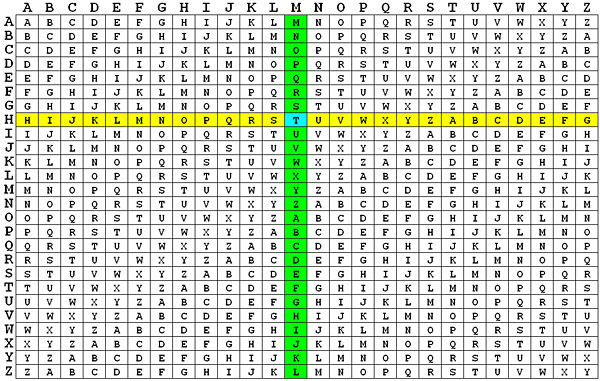
\includegraphics[scale=0.6]{./pics/vig}
\caption{Vigenère table}
\end{figure}
The above image of the Vigenère table was taken from a website authored by \textsl{Dr. C.-K. Shene a professor in the Department of Computer Science at Michigan Technological University} (circa. 2014) available at \url{https://pages.mtu.edu/~shene/NSF-4/Tutorial/VIG/Vig-Base.html}
\section{Vernam Cipher}
The Vernam cipher is a One-Time pad cipher meaning that the key used is only ever used once and never again. It makes use of the positional values of each letter in the alphabet and adds the plaintext to the key with these and then applies a modulo 26 calculation on the resulting values. The key used in this has certain stipulations, the first that it must be truly random (one that computers are somewhat able to do), it must also be as long as the given plain text and then ever be used again.
\subsection{Our Implementation}
Our Vernam algorithm implementation makes use of:
\begin{itemize}
\item a randomly generated key for use as the One-Time Pad.
\end{itemize}
\subsection{Algorithm Itself}
Our implementation of the Vernam cipher is practically the same as it is described. We generate a random key to use only once per encryption, add it numerically to the plaintext or file contents as integers (which represent the bytes) and then decrypt it by subtracting that key again. The text "mode" works as it should, adding the numerical values of the letters' position in the alphabet with those of the random key. However, due to the restrictions placed upon working with file contents while using Python (being unable to change the data type from integer representations of bytes) we simply add the random key as with the text (the exception being that the file's is generated differently as described below) instead of using the XOR function some digital implementations make use of.
\subsection{The One-Time Pad Random Key Generator}
Using python's random library, a key the length of whatever input the algorithm recieves is generated by using;
\begin{itemize}
\item the \texttt{randrange(65,91)} function, or all capital letter's ASCII values, for text encryption as a string, and
\item the \texttt{randrange(0,256)} function, or all possible character's ASCII values, for file encryption as an array of integers.
\end{itemize}
That is to say, it is a key that can consist of some/all 255 ASCII characters in numerical form. This key is then used in a further calculation on the once encrypted data as follows:
\\
For text encryption we make use of the following formula:\\
\texttt{EncryptedValue = (textASCII\_Value[ i ] + randomKeyASCII\_Value[ i ]\% 26) + 65}\\
(65 is the ASCII value of A)\\
And with file encryption we made use of the following formula:\\
\texttt{EncryptedValue = fileDataASCII\_Value[ i ] + randomKeyASCII\_Value[ i ] \% 256}\\
(Taken under modulo256 as character ASCII values are limited to this range)
\section{Transposition Cipher}
A transposition cipher is a means of encryption by which the plaintext characters are shifted according to a regular system. As such, the order of the plaintext is simply reordered. There are also several different methods of doing this, such as the Columnar Transposition which reads the columns in order of the key's character values (i.e. a=1, b=2, and so on). Others involve some form of distortion by adding some spaces or other characters to further mix up the plain text.
\subsection{Our Implementation}
Our Transposition algorithm implementation makes use of:
\begin{itemize}
\item a key checking function, and
\item a function to convert a string, or array depending on the "mode", into a matrix.
\end{itemize}
\subsection{The Algorithm Itself}
Before explaining the "formatting" methods used in this implementation of the transposition cipher, we explain which transposition method we made use of. The transposition cipher used is the "\textsl{rotate 90 degrees}" variant where the encrypted data is created by reading from a matrix depth-wise through all the columns. To achieve this digitally without any "out of index errors", the matrix is also padded with additional values depending on the "mode" during the matrix formulation function.
\subsection{The Key Check}
As some transposition models make use of an integer value while others a string we decided that ours would accept both:
\begin{itemize}
\item In the event an integer is entered, it would stipulate he number of columns within the matrix.
\item If a string of characters/letters/special characters/etc. is entered then this function would return the length of that string as the stipulation for the amount of columns in the matrix.
\end{itemize}
As our front-end makes use of Django's text fields to capture user input, we iterate over each element in the user given key and if all items are found to have the ASCII values of numbers, it is changed from a numerical string to an integer to be used.
(It should be noted that this function is also used in our "homebrew" algorithm due to the need to have an integer-based key)
\subsection{The Matrix Formulation}
We have two versions of this function for use:
\begin{itemize}
\item One for text encryption and decryption, and
\item One for file encryption and decryption.
\end{itemize}
The reason for this is due to the padding used in this implementation as we cannot pad a files contents with anything other than bytes and as such:
\begin{itemize}
\item For text we pad with the ("") character; essentially nothing but adding to the size of the matrix as ("") will have no affect on a string regardless of where it is padded.
\item For files we pad the remaining spaces with the last byte accessed - repeating it until the required size is reached.
\end{itemize}
Regardless of which is used, they both return a matrix (or technically a list of lists).
\subsection{Removal of padding}
Whereas the text version of this transposition essentially pads nothing, the file version pads actual values which must be removed during decryption to return usable "plaintext" file data. To accomplish this we had to store the original file length for use. From a back-end perspective, and when encrypting and then decrypting one file a a time, it was enough to store this length as another variable. However, as a user can encrypt multiple files before decrypting one, we needed a way to tie the original file content's length to its' encrypted version. We accomplished this by sorting the length as an additional array within the encrypted file through the following logic:
\begin{itemize}
\item As the length of a files contents' will almost definitely be greater than 255 (the maximum ASCII value) for all but the simplest files, we need to store this integer value as separate bytes for each digit in the number to not exceed this value.
\item We then took the length of this number (as it is impossible for it to reach 255 digits long as the largest number a computer can store, $2^31 - 1$, is only ten digits long).
\item Therefore, the first byte of the encrypted file contents is the number of times the array of bytes must be popped to be solely "ciphertext" again, still with padding, and to acquire the original length.
\item Finally, after the content has been decrypted, we pop() from the back equal to the difference of the matrices full length and the original length to remove all padding bytes.
\end{itemize}
\section{J\&A Homebrew Algorithm}
Our "Homebrew" algorithm makes use of:
\begin{itemize}
\item a mathematical calculation to increase the confusion aspect of the cipher text, and
\item a randomly generated key of all possible unicode/ASCII values to further enhance the confusion and diffusion aspects.
\end{itemize}
\subsection{The Mathematics}
With the use of a python mathematics library, such as the simple "math" module or NumPy, this calculation can be quite complex provided the programmer's mathematical knowledge is sufficient. One limitation this algorithm has is that, for files, no multiplication or division can be used as it changes the byte content between a float and an integer which causes it to loose its encoding type. Another is that no mathematical functions that returns multiple values can be used - such as a square root function returning both the positive and negative roots. The integer key a user provides is what is used in these calculations.
\\
As such, for the text encryption we made use of the following formula:\\
\texttt{encryptedValue = (key x plainTextASCII\_Value[ i ]) - key}\\
And with the aforementioned restrictions on file encryption we made use of the following formula:\\
\texttt{encryptedValue = (key x byteASCII\_Value[ i ]) - key}\\
The decryption of this aspect of the algorithm just takes the inverse of these mathematical calculations.
\subsection{Secondary Random Key}
Using python's random library, a key the length of whatever input the algorithm receives is generated by using;
\begin{itemize}
\item the \texttt{randrange(65,91)} function, or all capital letter's ASCII values, for text encryption, and
\item the randrange(32,256) function, or all possible character's ASCII values, for file encryption.
\end{itemize}
That is to say, it is a key that can consist of some/all 255 ASCII characters in numerical form. This key is then used in a further calculation on the once encrypted data as follows:\\\\
For text encryption we make use of the following formula:\\
\texttt{againEncryptedValue = encryptedValue[ i ] + randomKeyASCII\_Value[ i ]}\\
And with the aforementioned restrictions on file encryption we made use of the following formula:\\
\texttt{againEncryptedValue = (encryptedValue[ i ] + randomKeyASCII\_Value[ i ]) \% 256}\\
(Taken under modulo256 as character ASCII values are limited to this range)\\
The decryption of this aspect of the algorithm again just takes the inverse of these mathematical calculations.
\subsection{The Diffusion Aspect}
As the aforementioned random key is needed for decryption, it is actually included in the cipher text or encrypted file in a manner to increase diffusion of the encrypted data. As with the mathematical calculations, it depends on how a programmer wishes to diffuse the key. With this implementation, we have added it as the first half of the encrypted data - which is not too secure now that it's been disclosed :p
In the decryption of the encrypted file or cipher text:
\begin{itemize}
\item The first half is read as the key, and
\item The remaining contents as the encrypted file data or cipher text.
\end{itemize}
\chapter{Installation and setup}
\section{Project files}
The project files can be found on the following GitHub link:\\
\url{https://github.com/AM-ops/SecurityProject}
\\\\This was our main code repository. We both have been updating the code as we went along and added details and bug fixes to the project.\\\\
To copy the code to your own machine, follow the following steps:
\begin{enumerate}
\item Make sure Git is installed. If not it can be downloaded from here:\\
\url{https://git-scm.com/}
\item Create an empty directory where the code can be copied to
\item Run the following command:
\begin{minted}
[
frame=lines,
framesep=2mm,
baselinestretch=1.2,
bgcolor=LightApricot,
fontsize=\footnotesize,
]
{Shell}
git clone https://github.com/AM-ops/SecurityProject.git
\end{minted}
\end{enumerate}
\section{Virtual Environment}
There are multiple advantages of using virtual environments when creating software. The primary reason being we create a layer of separation and abstraction between our host machine's files and our software project.\\\\
We made use of a Python virtual environment which was handled by Anaconda. This can be downloaded from the following link:\\
\url{https://www.anaconda.com/products/individual}
\subsection{Creating a virtual environment}
Once Anaconda was installed the following commands were run in the terminal to create a virtual environment called \texttt{myDjangoEnv}.
\begin{minted}
[
frame=lines,
framesep=2mm,
baselinestretch=1.2,
bgcolor=LightApricot,
fontsize=\footnotesize,
]
{Shell}
conda create --name myDjangoEnv
\end{minted}
Depending on the version of Anaconda installed you might have to use a leading underscore on Windows machines. The same will apply for commands further down. Below is a demonstration.
\begin{minted}
[
frame=lines,
framesep=2mm,
baselinestretch=1.2,
bgcolor=LightApricot,
fontsize=\footnotesize,
]
{Shell}
_conda create --name myDjangoEnv
\end{minted}
\subsection{Listing virtual environments}
To list all virtual environments on your host machine run the following command.
\begin{minted}
[
frame=lines,
framesep=2mm,
baselinestretch=1.2,
bgcolor=LightApricot,
fontsize=\footnotesize,
]
{Shell}
conda info --envs
\end{minted}
or
\begin{minted}
[
frame=lines,
framesep=2mm,
baselinestretch=1.2,
bgcolor=LightApricot,
fontsize=\footnotesize,
]
{Shell}
conda env list
\end{minted}
\subsection{Deleting a virtual environment}
To delete a virtual environment run the following commands.
\begin{minted}
[
frame=lines,
framesep=2mm,
baselinestretch=1.2,
bgcolor=LightApricot,
fontsize=\footnotesize,
]
{Shell}
conda remove --name <name_of_virtual_environment> --all
\end{minted}
or
\begin{minted}
[
frame=lines,
framesep=2mm,
baselinestretch=1.2,
bgcolor=LightApricot,
fontsize=\footnotesize,
]
{Shell}
conda env remove --name <name_of_virtual_environment>
\end{minted}
\subsection{Activating and deactivating virtual environments}
To activate an environment run the following commands for Windows.
\begin{minted}
[
frame=lines,
framesep=2mm,
baselinestretch=1.2,
bgcolor=LightApricot,
fontsize=\footnotesize,
]
{Shell}
conda activate <name_of_virtual_environment>
\end{minted}
For Linux and MacOS the command is as follows.
\begin{minted}
[
frame=lines,
framesep=2mm,
baselinestretch=1.2,
bgcolor=LightApricot,
fontsize=\footnotesize,
]
{Shell}
source activate <name_of_virtual_environment>
\end{minted}
Once the environment is activated your terminal should change. By default, the active environment, is shown in parentheses () or brackets [] at the beginning of your command prompt as shown below.
\begin{minted}
[
frame=lines,
framesep=2mm,
baselinestretch=1.2,
bgcolor=LightApricot,
fontsize=\footnotesize,
]
{Shell}
(<name_of_virtual_environment>) >_
\end{minted}
Depending on your version of Anaconda to deactivate your environment the commands for Windows is.
\begin{minted}
[
frame=lines,
framesep=2mm,
baselinestretch=1.2,
bgcolor=LightApricot,
fontsize=\footnotesize,
]
{Shell}
deactivate
\end{minted}
or
\begin{minted}
[
frame=lines,
framesep=2mm,
baselinestretch=1.2,
bgcolor=LightApricot,
fontsize=\footnotesize,
]
{Shell}
conda deactivate
\end{minted}
For Linux and MacOS the command will be
\begin{minted}
[
frame=lines,
framesep=2mm,
baselinestretch=1.2,
bgcolor=LightApricot,
fontsize=\footnotesize,
]
{Shell}
source deactivate
\end{minted}
\subsection{Listing Packages installed}
To list all the packages you have installed in an environment there are two methods of listing them.
First, if the environment is not activated run the following.
\begin{minted}
[
frame=lines,
framesep=2mm,
baselinestretch=1.2,
bgcolor=LightApricot,
fontsize=\footnotesize,
]
{Shell}
conda list -n <name_of_virtual_environment>
\end{minted}
Secondly, if the environment is activated, then simply run the following.
\begin{minted}
[
frame=lines,
framesep=2mm,
baselinestretch=1.2,
bgcolor=LightApricot,
fontsize=\footnotesize,
]
{Shell}
conda list
\end{minted}
\subsection{Using pip}
Due to the fact that Python is being used for the project it is always necessary to make sure \texttt{pip} is installed and functioning. If it is not then run the following commands.
\begin{minted}
[
frame=lines,
framesep=2mm,
baselinestretch=1.2,
bgcolor=LightApricot,
fontsize=\footnotesize,
]
{Shell}
conda install -n <name_of_virtual_environment> pip
\end{minted}
\section{Frameworks and other packages}
\subsection{Django}\label{dj}
The primary framework used for development in this project was \texttt{Django}. This is a python based Web framework. The documentation for it can be found here:\\
\url{https://docs.djangoproject.com/en/3.2/}
\subsection{Bootstrap}\label{bs}
Bootstrap is Cascading Style Sheets (CSS) Framework which allows for simple, elegant, and responsive Graphical User Interfaces to be developed for the Web. The documentation for it can be found here:\\
\url{https://getbootstrap.com/docs/5.0/getting-started/introduction/}\\\\
For a more seamless integration of Bootstrap with the \texttt{Django} Framework an additional package called \texttt{django-crispy-forms} was also installed. Its documentation ca be found here:\\
\url{https://django-crispy-forms.readthedocs.io/en/latest/}
\subsection{Miscellaneous}
For typesetting of this documentation, \hologo{LaTeX} was utilised. Additionally, a \hologo{LaTeX} package called \texttt{minted} was used to typeset code in this documentation. Its homepage is located at: \url{https://www.ctan.org/pkg/minted}\\\\
To typeset directory structures in a tree-like manner the \hologo{LaTeX} package \texttt{dirtree} was used. Its homepage can be found at: \url{https://ctan.org/pkg/dirtree}\\\\
To typeset quotations for the Reflection section the \hologo{LaTeX} package \texttt{csquotes} was used. Its homepage can bee found at: \url{https://ctan.org/pkg/csquotes?lang=en}\\\\
Lastly, to typeset code within the HTML pages of our project the JavaScript library called \texttt{Rainbow} was implemented. The GitHub link for that is located at:\\
\url{https://github.com/ccampbell/rainbow}
\chapter{Programming of artefact}
\section{Development Tools}
\subsection{Operating Systems}
The primary systems on which development was done was Linux and Windows 10. The same systems where utilised for testing and bug fixing purposes.
\subsection{IDEs}
For the purposing of coding the following two Integrated Development Environments were used:
\begin{enumerate}
\item Atom. It can be downloaded from: \url{https://atom.io/}
\item Visual Studio Code, also known as VSCode. It can be downloaded from here: \url{https://code.visualstudio.com/}
\end{enumerate}
\subsection{Database Management Tools}
For the purposes of database management, TablePlus was the main software we utilised. It was used to see if our \texttt{Django} models and cryptographic schemes were correctly implemented. TablePlus can be downloaded from: \url{https://tableplus.com/}
\subsection{Hosting}
Due to a number of constraints we landed up running our project locally. The server was \texttt{localhost} and the port number was \texttt{8000}. Therefore the link where we ran our project was:
\url{http://127.0.0.1:8000}
\section{Prerequisites}
\subsection{Project and Package Initialisation}
\textsl{From here on we will refer to the working directory as the directory where the} \texttt{manage.py} \textsl{file is located. This file is created when the project is setup}\\\\
Before our \texttt{Django} project can be created we have to install all the packages mentioned above in Section \ref{dj} and \ref{bs}. A text file called \texttt{requirements.txt} was created which lists the 3 packages we need to install as shown below:
\begin{minted}
[
frame=lines,
framesep=2mm,
baselinestretch=1.2,
bgcolor=LightApricot,
fontsize=\footnotesize,
]
{Text}
django
django-crispy-forms
bootstrap4
\end{minted}
Thereafter the following command was run in the working directory.
\begin{minted}
[
frame=lines,
framesep=2mm,
baselinestretch=1.2,
bgcolor=LightApricot,
fontsize=\footnotesize,
]
{Shell}
pip install -r requirements.txt
\end{minted}
To start a \texttt{Django} project called \texttt{SecProj} the following command was run:
\begin{minted}
[
frame=lines,
framesep=2mm,
baselinestretch=1.2,
bgcolor=LightApricot,
fontsize=\footnotesize,
]
{Shell}
django-admin startproject SecProj
\end{minted}
Your directory should look like the following:
\dirtree{%
.1 /.
.2 manage.py.
.2 SecProj.
.3 \_\_init\_\_.py.
.3 settings.py.
.3 urls.py.
.3 asgi.py.
.3 wsgi.py.
}
\phantom{a}\\
\noindent To verify that your \texttt{Django} project is working run the following command in your working directory:
\begin{minted}
[
frame=lines,
framesep=2mm,
baselinestretch=1.2,
bgcolor=LightApricot,
fontsize=\footnotesize,
]
{Shell}
python manage.py runserver
\end{minted}
You should see the following if you open the link: \url{http://127.0.0.1:8000}
\begin{figure}[H]
\centering
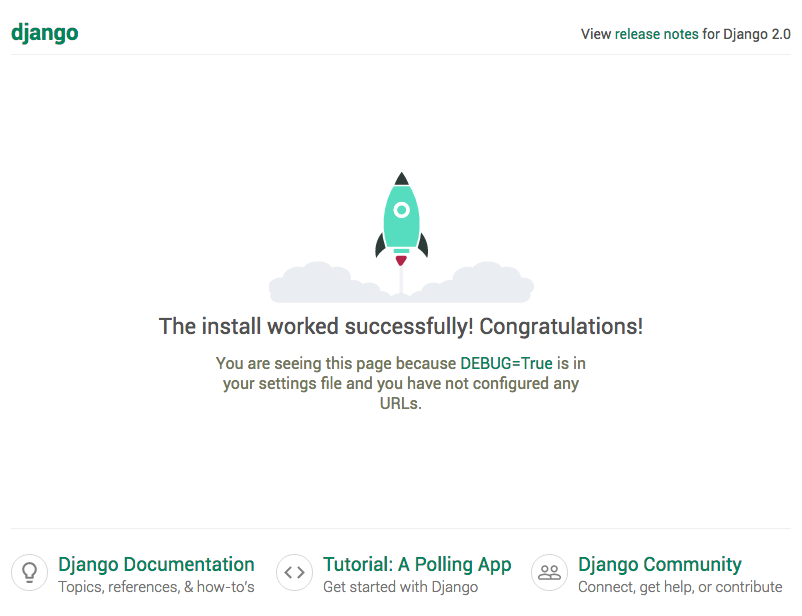
\includegraphics[scale=0.3]{./pics/home}
\caption{Default Homepage of a new Django Project}
\end{figure}
\noindent Now that your \texttt{Django} project is up and running it is time to create a \texttt{Django} 'App' within this project. This App is where we implemented our cryptographic schemes and the bulk of our project. We called our App \texttt{SecApp} and the command to run in your working directory is as follows:
\begin{minted}
[
frame=lines,
framesep=2mm,
baselinestretch=1.2,
bgcolor=LightApricot,
fontsize=\footnotesize,
]
{Shell}
python manage.py startapp SecApp
\end{minted}
Your directory should now look like the following:
\dirtree{%
.1 /.
.2 manage.py.
.2 SecProj.
.3 \_\_init\_\_.py.
.3 settings.py.
.3 urls.py.
.3 asgi.py.
.3 wsgi.py.
.2 SecApp.
.3 \_\_init\_\_.py.
.3 admin.py.
.3 apps.py.
.3 migrations.
.4 \_\_init\_\_.py.
.3 models.py.
.3 tests.py.
.3 views.py.
}
\subsection{Settings and Admin}
The following changes were added to the \texttt{settings.py} file. The whole file is not shown below.
\begin{minted}
[
frame=lines,
framesep=2mm,
baselinestretch=1.2,
bgcolor=LightApricot,
fontsize=\footnotesize,
linenos,
breaklines,
]
{Python}
from pathlib import Path
import os

# Build paths inside the project like this: BASE_DIR / 'subdir'.
BASE_DIR = Path(__file__).resolve().parent.parent
TEMPLATE_DIR = os.path.join(BASE_DIR, 'templates')

# Application definition

INSTALLED_APPS = [
    'django.contrib.staticfiles',
    'bootstrap4',
    'SecProj',
    'SecApp',
    'accounts',
    'crispy_forms',
]
CRISPY_TEMPLATE_PACK = 'bootstrap4'

ROOT_URLCONF = 'SecProj.urls'
TEMPLATES = [{'DIRS': [TEMPLATE_DIR]}]

# Static files (CSS, JavaScript, Images)
# https://docs.djangoproject.com/en/3.1/howto/static-files/

STATIC_URL = '/static/'
STATICFILES_DIR = [os.path.join(BASE_DIR,'static')]
STATICFILES_DIRS = [
    os.path.join(BASE_DIR, "static"),
]
LOGIN_REDIRECT_URL = 'success'
LOGOUT_REDIRECT_URL = 'thanks'
MEDIA_URL = '/media/'
MEDIA_ROOT = os.path.join(BASE_DIR, 'media')
\end{minted}
To create a superuser to handle \texttt{Django} administration run the following commands and follow the prompts:
\begin{minted}
[
frame=lines,
framesep=2mm,
baselinestretch=1.2,
bgcolor=LightApricot,
fontsize=\footnotesize,
]
{Shell}
python manage.py createsuperuser
\end{minted}
The link for \texttt{Django} admininstration for the project is: \url{http://127.0.0.1:8000/admin}
\section{Models}
A workflow diagram of how the backend and frontend were created is given below:\\\\
\begin{center}
\begin{tikzpicture}[node distance=2cm]
\node (start) [startstop] {Beginning};
%\node (in1) [io, below of=start] {Input};
\node (pro1) [process, below of=start] {Create \texttt{Models}};
\node (pro6) [process, left of=pro1, xshift=-4cm] {Create Algorithms};
\node (pro7) [process, right of=pro1, xshift=4cm] {Create File and Text Management methods};
\node (pro2) [process, below of=pro1] {Create \texttt{ModelForms}};
\node (pro3) [process, below of=pro2] {Create \texttt{Views}};
\node (pro4) [process, below of=pro3] {Create \texttt{Templates}};
\node (pro5) [process, below of=pro4] {Add urls};
%\node (dec1) [decision, below of=pro1, yshift=-0.5cm] {Decision 1};
%
%\node (pro2a) [process, below of=dec1, yshift=-0.5cm] {Process 2a};
%\node (pro2b) [process, right of=dec1, xshift=2cm] {Process 2b};
%\node (out1) [io, below of=pro2a] {Output};
\node (stop) [startstop, below of=pro5] {Ending, and Testing};
\draw [arrow] (start) -| (pro6);
\draw [arrow] (start) -| (pro7);
\draw [arrow] (start) -- (pro1);
\draw [arrow] (pro1) -- (pro2);
\draw [arrow] (pro6) -- (pro1);
\draw [arrow] (pro7) -- (pro1);
\draw [arrow] (pro2) -- (pro3);
\draw [arrow] (pro3) -- (pro4);
\draw [arrow] (pro4) -- (pro5);
\draw [arrow] (pro5) -- (stop);
%\draw [arrow] (pro1) -- (dec1);
%\draw [arrow] (dec1) -- (pro2a);
%\draw [arrow] (dec1) -- (pro2b);
%\draw [arrow] (dec1) -- node[anchor=east] {yes} (pro2a);
%\draw [arrow] (dec1) -- node[anchor=south] {no} (pro2b);
%\draw [arrow] (pro2b) |- (pro1);
%\draw [arrow] (pro2a) -- (out1);
%\draw [arrow] (out1) -- (stop);
\end{tikzpicture}
\end{center}
The process of creating models was identical for all that were created, therefore for the purpose of brevity we will only look at one text, and one file example. The example will be of the models implemented for the Vigenère cryptographic scheme.\\\\
The model for Text Encryption and Decryption with the Vigenère cipher looks exactly the same with a few small differences. Below is the code for Text Encryption and Decryption. This code was added to the \texttt{models.py} file.\\\\
A few notes to mention before we move to the code:
\begin{itemize}
\item The \texttt{TextField} was a \texttt{ModelField} used due to its capability to store large strings of textual data. It is synonymous with \texttt{nvarchar} or \texttt{varchar} in other DBMSs.
\end{itemize}
\begin{minted}
[
frame=lines,
framesep=2mm,
baselinestretch=1.2,
bgcolor=LightApricot,
fontsize=\footnotesize,
linenos,
]
{Python}
class VigTextEnc(models.Model):
    user = models.ForeignKey(User, on_delete=models.CASCADE, null=True, blank=True)
    plaintext = models.TextField(null=False, default='')
    ciphertext = models.TextField(null=False,default='')
    key = models.TextField(null=False,default='')
    description = models.TextField(default='Vigenere Text Encryption')

    def save(self, *args, **kwargs):
        self.enc()
        super().save(*args, **kwargs)

    def enc(self, *args, **kwargs):
        self.ciphertext = algorithms.Vigenere_TEXT_Encryption(self.plaintext,self.key)

    def get_absolute_url(self):
        return reverse('SecApp:VigTextEnc_detail', kwargs={'pk':self.pk})

class VigTextDec(models.Model):
    user = models.ForeignKey(User, on_delete=models.CASCADE, null=True, blank=True)
    plaintext = models.TextField()
    ciphertext = models.TextField()
    key = models.TextField(null=False,default='')
    description = models.TextField(default='Vigenere Text Decryption')

    def save(self, *args, **kwargs):
        self.dec()
        super().save(*args, **kwargs)

    def dec(self, *args, **kwargs):
        self.plaintext = algorithms.Vigenere_TEXT_Decryption(self.ciphertext,self.key)

    def get_absolute_url(self):
        return reverse('SecApp:VigTextDec_detail', kwargs={'pk':self.pk})
\end{minted}
The model for File Encryption and Decryption with the Vigenère cipher looks exactly the same with a few small differences. Below is the code.\\\\
A few notes to mention before we move to the code:
\begin{itemize}
\item The \texttt{FileField} was a \texttt{ModelField} used due to its capability to store \textbf{metadata} about a file. So in other words its format, url, and path of where the file is located. \item It stores references that point to a certain object after it is uploaded and saved under the \texttt{/media/} directory.
\end{itemize}
\begin{minted}
[
frame=lines,
framesep=2mm,
baselinestretch=1.2,
bgcolor=LightApricot,
fontsize=\footnotesize,
linenos,
breaklines
]
{Python}
class VigFileEnc(models.Model):
    user = models.ForeignKey(User, on_delete=models.CASCADE, null=True, blank=True)
    plaintext = models.FileField(upload_to='', blank=True)
    ciphertext = models.TextField(default='')
    description = models.TextField(default='Vigenere File Encryption')
    key = models.TextField(blank=True,default='')
    ext = models.CharField(max_length=10)

    def save(self, *args, **kwargs):
        super().save(*args, **kwargs)
        self.enc()
        super().save(*args, **kwargs)
    def enc(self, *args, **kwargs):
        THIS_FOLDER = os.path.dirname(os.path.abspath(settings.MEDIA_ROOT))
        new_path = os.path.join(THIS_FOLDER, 'media')
        pt = str(self.plaintext.path)
        plainData = algorithms.fileToByteString(pt)
        cipherData = algorithms.Vigenere_FILE_Encryption(plainData,self.key)
        self.ciphertext = algorithms.byteStringToFile(cipherData, os.path.join(new_path, 'newfile_vig_enc.{0}'.format(self.ext)))
    def get_absolute_url(self):
        return reverse('SecApp:VigFileEnc_detail', kwargs={'pk':self.pk})

class VigFileDec(models.Model):
    user = models.ForeignKey(User, on_delete=models.CASCADE, null=True, blank=True)
    plaintext = models.TextField(default='')
    ciphertext = models.FileField(upload_to='', blank=True)
    description = models.TextField(default='Vigenere File Decryption')
    key = models.TextField(blank=True,default='')
    ext = models.CharField(max_length=10)

    def save(self, *args, **kwargs):
        super().save(*args, **kwargs)
        self.dec()
        super().save(*args, **kwargs)
    def dec(self, *args, **kwargs):
        THIS_FOLDER = os.path.dirname(os.path.abspath(settings.MEDIA_ROOT))
        new_path = os.path.join(THIS_FOLDER, 'media')
        pt = str(self.ciphertext.path)
        plainData = algorithms.fileToByteString(pt)
        cipherData = algorithms.Vigenere_FILE_Decryption(plainData,self.key)
        self.plaintext = algorithms.byteStringToFile(cipherData, os.path.join(new_path, 'newfile_vig_dec.{0}'.format(self.ext)))
    def get_absolute_url(self):
        return reverse('SecApp:VigFileDec_detail', kwargs={'pk':self.pk})
\end{minted}
Once the \texttt{Models} are finalised we can create the \texttt{ModelForms}. Below is the snippet of code for the \texttt{ModelForms} that use the \texttt{Models} shown above.
 \begin{minted}
[
frame=lines,
framesep=2mm,
baselinestretch=1.2,
bgcolor=LightApricot,
fontsize=\footnotesize,
linenos,
breaklines
]
{Python}
class VigTextEncModelForm(ModelForm):
    class Meta:
        model = VigTextEnc
        fields = ['plaintext','key']
        labels = {
        "plaintext": "Text to Encrypt",
        "key": "Key",
        }
        widgets = {
        'plaintext': forms.Textarea(attrs={'class':'form-control', 'placeholder':'Enter text here','rows':5,}),
        'key': forms.Textarea(attrs={'class':'form-control', 'placeholder':'Enter ONLY Alphabet Letters','rows':5,}),
        }

        def __init__(self, *args, **kwargs):
            super().__init__(*args, **kwargs)

class VigTextDecModelForm(ModelForm):
    class Meta:
        model = VigTextDec
        fields = ['ciphertext','key']
        labels = {
        "ciphertext": "Text to Decrypt",
        'key':'Key',
        }
        widgets = {
        'ciphertext': forms.Textarea(attrs={'class':'form-control', 'placeholder':'Enter text here','rows':5,}),
        'key': forms.Textarea(attrs={'class':'form-control', 'placeholder':'Enter ONLY Alphabet Letters','rows':5,}),
        }

        def __init__(self, *args, **kwargs):
            super().__init__(*args, **kwargs)
\end{minted}
The \texttt{ModelForms} make it easier to implement a HTML form, thereby streamlining the process. Using \texttt{ModelForms} we can specify exactly what fields should be displayed on a form, which ones are mandatory to fill in, which ones are optional, as well as specify additional information to make the User Experience more pleasant for anyone that uses the program.
\section{Views}
Once the \texttt{Models} and \texttt{ModelForms} are completed we can move onto the Views. The primary ones that are used are the \texttt{CreateView}, \texttt{DetailView}, and the \texttt{TemplateView}. These are all classes that inherit from the parent \texttt{GenericView}.\\\\
Once again we will look at the Vigenère cipher and the models created for it and how they are integrated with the \texttt{Views}. Below is the snippet of code for the \texttt{CreateView}.
 \begin{minted}
[
frame=lines,
framesep=2mm,
baselinestretch=1.2,
bgcolor=LightApricot,
fontsize=\footnotesize,
linenos,
breaklines
]
{Python}
class VigOverviewPage(TemplateView):
    template_name = 'SecApp/vig/overview.html'
    
class VigTextEncCreate(LoginRequiredMixin,CreateView):
    form_class = forms.VigTextEncModelForm
    template_name = 'SecApp/vig/vig_enc_create_form.html'
    model = models.VigTextEnc

    def form_valid(self, form):
        self.object = form.save(commit=False)
        self.object.user = self.request.user
        self.object.save()
        return super().form_valid(form)

class VigTextDecCreate(LoginRequiredMixin,CreateView):
    form_class = forms.VigTextDecModelForm
    template_name = 'SecApp/vig/vig_dec_create_form.html'
    model = models.VigTextDec

    def form_valid(self, form):
        self.object = form.save(commit=False)
        self.object.user = self.request.user
        self.object.save()
        return super().form_valid(form)

class VigFileEncCreate(LoginRequiredMixin,CreateView):
    form_class = forms.VigFileEncModelForm
    template_name = 'SecApp/vig/vig_enc_create_file.html'
    model = models.VigFileEnc

class VigFileDecCreate(LoginRequiredMixin,CreateView):
    form_class = forms.VigFileDecModelForm
    template_name = 'SecApp/vig/vig_dec_create_file.html'
    model = models.VigFileDec
\end{minted}
Next we can create the \texttt{DetailView} for the same \texttt{Models} mentioned above.
 \begin{minted}
[
frame=lines,
framesep=2mm,
baselinestretch=1,
bgcolor=LightApricot,
fontsize=\footnotesize,
linenos,
breaklines
]
{Python}
class VigTextEncDetailView(LoginRequiredMixin,DetailView):
    model = models.VigTextEnc
    context_object_name = 'detail'
    template_name = 'SecApp/vig/vig_text_enc_detail.html'

class VigTextDecDetailView(LoginRequiredMixin,DetailView):
    model = models.VigTextDec
    context_object_name = 'detail'
    template_name = 'SecApp/vig/vig_text_dec_detail.html'
    
class VigFileEncDetailView(LoginRequiredMixin,DetailView):
    model = models.VigFileEnc
    context_object_name = 'detail'
    template_name = 'SecApp/vig/vig_file_enc_detail.html'

class VigFileDecDetailView(LoginRequiredMixin,DetailView):
    model = models.VigFileDec
    context_object_name = 'detail'
    template_name = 'SecApp/vig/vig_file_dec_detail.html'
\end{minted}
\section{Templates}
We are almost complete with our implementation. We now have to create \texttt{Templates} that link up with the \texttt{Views} created above. Below is a snippet of code for Vigenère Text Encryption \texttt{View}
 \begin{minted}
[
frame=lines,
framesep=2mm,
baselinestretch=1.1,
bgcolor=LightApricot,
fontsize=\footnotesize,
linenos,
breaklines
]
{html+django}


Fill in text




<div class="container">
  <div class="container m-5 p-3">
    <h1 style="text-align: center;">Text Encryption with Vigen&egrave;re</h1>
    <form method="post" class="form m-5">
      
      {{ form | crispy}}
      <div style="text-align: center;">
      <input type="submit" value="Encrypt" class="btn btn-success">
      <a class="btn btn-outline-success" href="">Go Back</a>
      </div>
    </form>
  </div>
</div>
\end{minted}
\section{URLs}
Lastly, we have to add the URLs for the \texttt{Views} and \texttt{Templates} created above. The code is added to the \texttt{urls.py} file. For each \texttt{View} that was created a separate URL had to be added. Below is the snippet.
 \begin{minted}
[
frame=lines,
framesep=2mm,
baselinestretch=1.2,
bgcolor=LightApricot,
fontsize=\footnotesize,
linenos,
breaklines,
]
{Python}
from django.conf.urls import url
from . import views

app_name = 'SecApp'

urlpatterns = [
url(r'^vig/$',views.VigOverviewPage.as_view(),name='vig_overview'),
    url(r'^vig/text/create/enc$',views.VigTextEncCreate.as_view(),
    name='vig_text_create_enc'),
    url(r'^vig/text/create/dec$',views.VigTextDecCreate.as_view(),
    name='vig_text_create_dec'),
    url(r'^vig/file/create/enc$',views.VigFileEncCreate.as_view(),
    name='vig_file_create_enc'),
    url(r'^vig/file/create/dec$',views.VigFileDecCreate.as_view(),
    name='vig_file_create_dec'),
    url(r'vig/text/enc/(?P<pk>\d+)/$',views.VigTextEncDetailView.as_view(),
     name='VigTextEnc_detail'),
    url(r'vig/text/dec/(?P<pk>\d+)/$',views.VigTextDecDetailView.as_view(),
     name='VigTextDec_detail'),
    url(r'vig/file/enc/(?P<pk>\d+)/$',views.VigFileEncDetailView.as_view(),
     name='VigFileEnc_detail'),
    url(r'vig/file/dec/(?P<pk>\d+)/$',views.VigFileDecDetailView.as_view(),
     name='VigFileDec_detail'),
    ]
\end{minted}
\section{Migrations}
To finally run the program we have to run a few commands. The first make our migrations, the second migrates those changes to our local SQLite database, and the last command runs our server locally.
 \begin{minted}
[
frame=lines,
framesep=2mm,
baselinestretch=1.1,
bgcolor=LightApricot,
fontsize=\footnotesize,
linenos,
breaklines
]
{Shell}
python manage.py makemigrations
python manage.py migrate
python manage.py runserver
\end{minted}
All these commands, and a few other commands were added to a \texttt{script.sh} file for Linux development and in a \texttt{script.bat} file for Windows development.
\section{Algorithms, File and Text Management Methods}
First we will display the code located in our \texttt{algorithms.py} file then we will discuss the methods in detail.
 \begin{minted}
[
frame=lines,
framesep=2mm,
baselinestretch=1.2,
bgcolor=LightApricot,
fontsize=\footnotesize,
linenos,
breaklines,
]
{Python}
#Cryptography Project for ITRI615
# J&A's Cryptography Project
import math
import random as r

#Formatting files
#for any type of file :D
def fileToByteString(file):
    byteStream =[]
    f = open(file, 'rb')
    fileData = f.read()
    fileData = bytearray(fileData)

    for item in fileData:
        byteStream.append(item)

    f.close()
    return byteStream

def byteStringToFile(byteStream,file):
    pathStr = str(file)
    f = open(file, 'wb')
    byteStream = bytearray(byteStream)
    f.write(byteStream)
    f.close()
    return pathStr

#Transposition
def keyCheck(key):
    check = True
    for item in key:
        if(not(ord(item) >= 48 and ord(item) <= 57)):
            check = False
    if(check):
        return int(key)
    else:
        return len(key)

#String to Matrix function
def StrToMatrix_TEXT(text,key):
    matrix = []
    row = []
    count = 0
    length = len(text)
    for item in text:
        row.append(item)
        count = count + 1
        length = length - 1
        if(count == key):
            matrix.append(row)
            row = []
            count = 0
        elif(length == 0):
            while(len(row)<key):
                row.append("")
            matrix.append(row)
    return matrix

def StrToMatrix_FILE(text,key):
    matrix = []
    row = []
    count = 0
    length = len(text)
    for item in text:
        row.append(item)
        count += 1
        length -= 1
        if(count == key):
            matrix.append(row)
            row = []
            count = 0
        elif(length == 0):
            while(len(row)<key):
                row.append(item)
            matrix.append(row)
    return matrix

#Text algoritms
def Transposition_TEXT_Encryption(message, key):
    key = keyCheck(key)
    matrix = StrToMatrix_TEXT(message, key)
    encryptedMessage = ""
    for j in range(0,key):
        for item in matrix:
            strList = str(item.pop(0))
            encryptedMessage = encryptedMessage+strList
    return encryptedMessage

def Transposition_TEXT_Decryption(encryptedMessage, key):
    key = keyCheck(key)
    numberColumns = math.ceil(len(encryptedMessage) / key)
    numberRows = key
    numberBlanks = (numberColumns * numberRows) - len(encryptedMessage)
    decryptedMessage = ['']*numberColumns
    col,row = 0,0

    for item in encryptedMessage:
        decryptedMessage[col] += item
        col += 1
        if (col == numberColumns) or 
        (col == numberColumns - 1 and row >= numberRows - numberBlanks):
            col = 0
            row += 1
    return ''.join(decryptedMessage)

def Transposition_FILE_Encryption(message, key):
    key = keyCheck(key)
    matrix = StrToMatrix_FILE(message, key)
    encryptedMessage = []
    origLength = str(len(message))
    lenLen = len(origLength)
    encryptedMessage.append(lenLen)
    for i in range(0,lenLen):
        encryptedMessage.append(ord(origLength[i]))


    for j in range(0,key):
        for item in matrix:
            strList = item.pop(0)
            encryptedMessage.append(strList)
    return encryptedMessage

def Transposition_FILE_Decryption(message,key):
    key = keyCheck(key)

    lenLen = message.pop(0)
    origLengthARR = []
    for i in range(0,lenLen):
        strList = message.pop(0)
        origLengthARR.append(str(chr(strList)))
    origLengthSTR = ''.join(origLengthARR)
    origLength = int(origLengthSTR)

    numberColumns = math.ceil(len(message) / key)
    numberRows = key
    numberBlanks = (numberColumns * numberRows) - origLength
    matrix = StrToMatrix_FILE(message, numberColumns)
    decryptedMessageARR = []

    for j in range(0,numberColumns):
        for item in matrix:
            strList = item.pop(0)
            decryptedMessageARR.append(strList)

    for i in range(0,numberBlanks):
        decryptedMessageARR.pop(-1)

    returnMessage =[]
    for item in decryptedMessageARR:
        returnMessage.append(int(item))

    returnMessage = bytearray(returnMessage)

    return returnMessage

#Vignere

#Fixes key length to match size of message
def extendKeyLength(messageLength,key):
    keyLength = len(key)
    newKey = list(key)
    if messageLength == keyLength:
        return(key)

    else:
        for i in range(0,(messageLength - keyLength)):
            newKey.append(key[i % keyLength])
        return ("".join(newKey)).upper()

#Text algorithms
def Vigenere_TEXT_Encryption(message, key):
    message = message.upper()
    messageLength = len(message)
    encryptedMessage = []
    key = extendKeyLength(messageLength, key)
    for i in range(0,messageLength):
        if ord(message[i]) < 65 or ord(message[i]) > 90:
            encryptedMessage.append(message[i])
        else:
            newEncrypted = ord(message[i]) + ord(key[i])
            newEncrypted = newEncrypted % 26
            newEncrypted += ord('A') #gets ascii values back to "letters area"
            encryptedMessage.append(chr(newEncrypted))

    return "".join(encryptedMessage)

def Vigenere_TEXT_Decryption(encryptedMessage, key):
    decryptedMessage = []
    messageLength = len(encryptedMessage)
    key = extendKeyLength(messageLength, key)
    for i in range(0,messageLength):
        if ord(encryptedMessage[i]) < 65 or ord(encryptedMessage[i]) > 90:
            decryptedMessage.append(encryptedMessage[i])
        else:
            newDecrypted = (ord(encryptedMessage[i]) - ord(key[i])) % 26
            newDecrypted += ord('A')
            decryptedMessage.append(chr(newDecrypted))

    return "".join(decryptedMessage)

#File algortitms
def Vigenere_FILE_Encryption(message, key):
    messageLength = len(message)
    encryptedMessage = []
    key = extendKeyLength(messageLength, key)
    for i in range(0,messageLength):
            newEncrypted = ((message[i]) + ord(key[i])) % 256
            encryptedMessage.append(newEncrypted)

    return encryptedMessage

def Vigenere_FILE_Decryption(message, key):
    messageLength = len(message)
    decryptedMessage = []
    key = extendKeyLength(messageLength, key)
    for i in range(0,messageLength):
        newDecrypted = (message[i] - ord(key[i])) % 256
        decryptedMessage.append(newDecrypted)

    return decryptedMessage

#Vernam
#Key generators
def vernam_Key_Generator(messageLength):
    key = []
    for i in range(0,messageLength):
        char = chr(r.randrange(65,91))
        key.append(char)
    return ("".join(key)).upper()

def vernam_Key_Generator_FILE(messageLength):
    key = []
    for i in range(0,messageLength):
        char = chr(r.randrange(0,256))
        key.append(ord(char))
    return key

#Text algorithms
def Vernam_TEXT_Encryption(message):
    messageStrip = message.replace(" ","")
    messageStrip = messageStrip.upper()
    messageLength = len(messageStrip)
    key = vernam_Key_Generator(messageLength)
    encryptedMessage = "" + key
    encryptedMessage = list(encryptedMessage)
    for i in range(0,messageLength):
        newEncrypted = (ord(messageStrip[i]) + ord(key[i])) % 26
        newEncrypted += 65
        encryptedMessage.append(chr(newEncrypted))
    return "".join(encryptedMessage)

def Vernam_TEXT_Decryption(message):
    messageLength = int(len(message)/2)
    key = []
    baseMessage = []
    decryptedMessage = []

    for i in range(0,messageLength):
        key.append(message[i])
        baseMessage.append(message[(i+messageLength)])

    for j in range(0,messageLength):
        newDecrypted = (ord(baseMessage[j]) - ord(key[j])) % 26
        newDecrypted += 65
        decryptedMessage.append(chr(newDecrypted))

    return "".join(decryptedMessage)

#File algorithms
def Vernam_FILE_Encryption(message):
    messageLength = len(message)
    key = vernam_Key_Generator_FILE(messageLength)
    baseMessage = []
    encryptedMessage = []
    for j in key:
        encryptedMessage.append(j)
    for i in range(0,messageLength):
        newEncrypted = (message[i] + key[i]) % 256
        baseMessage.append(newEncrypted)


    encryptedMessage = [key,baseMessage]
    returnMessage = []
    for item in encryptedMessage:
        for thing in item:
            returnMessage.append(thing)

    return returnMessage

def Vernam_FILE_Decryption(message):
    messageLength = int(len(message)/2)
    key = []
    baseMessage = []
    decryptedMessage = []

    for i in range(0,messageLength):
        key.append(message[i])
        baseMessage.append(message[(i+messageLength)])

    for j in range(0,messageLength):
        newDecrypted = (baseMessage[j] - key[j]) % 256
        decryptedMessage.append(newDecrypted)

    return decryptedMessage

#Own algorithm
def own_TEXT_Encryption(message, key):
    key = keyCheck(key)
    messageLength = len(message)
    numericEncryptedValues = []
    for item in message:
        numeric = ord((item))
        mathPart = (((key*numeric)) - key)
        numericEncryptedValues.append(mathPart)

    randomKey = []
    for i in range(0,messageLength):
        num = r.randrange(32,256)
        randomKey.append(chr(num))

    encryptedMessage = []
    for i in range(0,messageLength):
        encryptedMessage.append(chr((numericEncryptedValues[i]+ord(randomKey[i]))))

    addedKey = ''.join(randomKey)
    strEncryptedMessage = ''.join(encryptedMessage)

    return (addedKey+strEncryptedMessage)

def own_TEXT_Decryption(message, key):
    key = keyCheck(key)
    messageLength = int(len(message)/2)
    encryptedMessage = []
    randomKey = []

    for i in range(0,messageLength):
        encryptedMessage.append(ord(message[i+messageLength]))
        randomKey.append(ord(message[i]))

    partA = []
    for j in range(0,messageLength):
        partA.append(chr((encryptedMessage[j]-randomKey[j])))

    decryptedMessage = []
    for item in partA:
        numeric = ord(item)
        unMathPart = ((numeric+key)/key)
        decryptedMessage.append(chr(int(unMathPart)))

    return ''.join(decryptedMessage)

def own_FILE_Encryption(message, key):
    key = keyCheck(key)
    messageLength = len(message)
    numericEncryptedValues = []
    for item in message:
        mathPart = (item - key)
        numericEncryptedValues.append(mathPart)

    randomKey = []
    for i in range(0,messageLength):
        num = r.randrange(0,256)
        randomKey.append(num)

    combined = []
    for i in range(0,messageLength):
        combined.append((numericEncryptedValues[i]+randomKey[i])%256)

    encryptedMessage = [randomKey,combined]
    returnMessage = []
    for item in encryptedMessage:
        for thing in item:
            returnMessage.append(thing)

    return returnMessage

def own_FILE_Decryption(message, key):
    key = keyCheck(key)
    messageLength = int(len(message)/2)
    encryptedMessage = []
    randomKey = []

    for i in range(0,messageLength):
        encryptedMessage.append(message[i+messageLength])
        randomKey.append(message[i])

    partA = []
    for j in range(0,messageLength):
        partA.append((encryptedMessage[j]-randomKey[j]))

    decryptedMessage = []
    for item in partA:
        unMathPart = (item+key)
        decryptedMessage.append(unMathPart%256)

    return decryptedMessage
\end{minted}
\texttt{fileToByteString()} Method\\
This method takes in a file/file path and reads it in binary mode. This data is then converted to a bytes array such that it can be worked on by other functions.
\\\\
\texttt{byteStringToFile()} Method\\
This function takes in an bytes array of decimal values  and writes them to the file/file path provided.\\\\
\texttt{keyCheck(key)} Method\\
This function takes the provided key and checks if it is a integer or string and if a string returns the length of it to use as a key.\\\\
\texttt{StrToMatrix\_TEXT()} Method\\
This function takes in a text string and a numerical key. The key is used to stipulate the number of desired columns in the matrix. The function then rearranges the string into the matrix and accordingly returns it. It also pads the last row if required.\\\\
\texttt{Transposition\_TEXT\_Encryption()} Method\\
This function takes in a string and a numerical key and passes them to \texttt{StrToMatrix\_TEXT()}. This function then applies a simple transposition cipher by reading the data from the matrix column wise.
\\\\
\texttt{Transposition\_TEXT\_Decryption()} Method\\
This function takes in a string and a numerical key. The function then uses various mathematical principles to work out how to read the encrypted text back; it does this by essentially transposing the matrix again. As such, it compiles a matrix to accomplish this and then returns a string through the .join() function.
\\\\
\texttt{StrToMatrix\_FILE()} Method\\
Works similar to \texttt{StrToMatrix\_TEXT()} with the exception of what is used as padding - a null byte transformed into an integer value; i.e. \texttt{ord("\textbackslash u0000")}.
\\\\
\texttt{Transposition\_FILE\_Encryption()} Method\\
Works similar to \texttt{Transposition\_TEXT\_Encryption()} with the exception of returning a numerical array instead of a string as well as taking in a byte array in place of a string.
\\\\
\texttt{Transposition\_FILE\_Decryption()} Method\\
Works similar to \texttt{Transposition\_TEXT\_Decryption()} with the exception of returning a numerical array instead of a string and removing the added padding as well as taking in a byte array in place of a string.
\\\\
\texttt{extendKeyLength()} Method\\
This function takes the length of the string given and the key to be used and ensures the key matches the length and if not duplicates it until it does. There is no need for a shortening function due to how the Vigenere Algorithm uses.
\\\\
\texttt{Vigenere\_TEXT\_Encryption()} Method\\
This function takes in a string and a key. It then converts the plaintext to uppercase letters. Instead of making use of a Vigenere Table - this function makes use of the numerical ASCII values of characters and adds them in modulo 26. It then adds the value of 65, or ord('A') to get all character values back to the range of letters and returns these as a string. It also includes a check to ignore any non-letter based characters as a Vigenere table is only alphabet letters.
\\\\
\texttt{Vigenere\_TEXT\_Decryption()} Method\\
Works similar to the encryption but instead subtracts the values before adding 65.
\\\\
\texttt{Vigenere\_FILE\_Encryption()} Method\\
Works as with Vigenere\_TEXT\_Encryption() but is applied within modulo 256 to encompass all possible characters as well as taking in a byte array in place of a string.
\\\\
\texttt{Vigenere\_FILE\_Decryption()} Method\\
Works as with \texttt{Vigenere\_TEXT\_Decryption()} but is applied within modulo 256 to encompass all possible characters as well as taking in a byte array in place of a string.
\\\\
The method of adding and subtracting numerical ASCII values has been found by us to consistently produce the same results as using a Vigenere table and as such was used as it would decrease look-up and computational time - especially on larger files.
\\\\
\texttt{vernam\_Key\_Generator()} Method\\
This function takes in the length of a message/string and produces a random string of characters (within the capital letter set) to be used in the encryption functions.
\\\\
\texttt{Vernam\_TEXT\_Encryption()} Method\\
This function takes in a message/string to be encrypted and calls \texttt{vernam\_Key\_Generator()} to create a unique one-time key. The ascii values of the message and key are added within modulo 26. The function then adds the required value to have the characters to be letter characters again and returns this as a string. Due to the random key generation, the key is stored as part of the resulting encrypted text.
\\\\
\texttt{Vernam\_TEXT\_Decryption()} Method\\
This function begins by separating the key from the encrypted text and then subtracts the values in modulo26, takes these values back to the range of letter characters and returns this as a string.
\\\\
\texttt{vernam\_Key\_Generator\_FILE()} Method\\
This function works similar to \texttt{vernam\_Key\_Generator()} except it generates an array of numerical values (between 0 and 255) as a key.
\\\\
\texttt{Vernam\_FILE\_Encryption()} Method\\
Works like \texttt{Vernam\_TEXT\_Encryption()} except it takes in a numerical array of byte values and is done within modulo256.
\\\\
\texttt{Vernam\_FILE\_Decryption()} Method\\
Works like \texttt{Vernam\_TEXT\_Decryption()} except it takes in a numerical array of byte values and is done within modulo256.
\\\\
\texttt{own\_TEXT\_Encryption()} Method\\
This function takes in a plaintext string and well as a integer key. The individual characters of the string are subjected to a mathematical calculation based on the provided key and added to an array. Afterwards, a randomly generated key of the same length is created consisting of values from 0 to 255 to be added to the array as well before being added to the array as well. A string result of these is then returned.
\\\\
\texttt{own\_TEXT\_Decryption()} Method\\
This function takes in a ciphertext string and a key. The cipher text is split into the encrypted text and a random key used in its' generation. The encrypted text is covered to numerical ascii values and have the random-key's values subtracted from it before having the inverse of a mathematical calculation based on the value of the key argument. This result is then concatenated and returned.
\\\\
\texttt{own\_FILE\_Encryption()} Method\\
Works very similar to \texttt{own\_TEXT\_Encryption()} except is takes in a byte array in place of a string and the values of the mathematical calculations are done in modulo256 to stay within the 0-255 byte limitations.
\\\\
\texttt{own\_FILE\_Decryption()} Method\\
Works very similar to \texttt{own\_TEXT\_Decryption()} except is takes in a byte array in place of a string and the values of the mathematical calculations are done in modulo256 to stay within the 0-255 byte limitations.
\chapter{User manual}
\section{Homepage}
The landing page for our site is located at \url{http://127.0.0.1:8000/} and look like the picture shown below:
\begin{figure}[H]
\centering
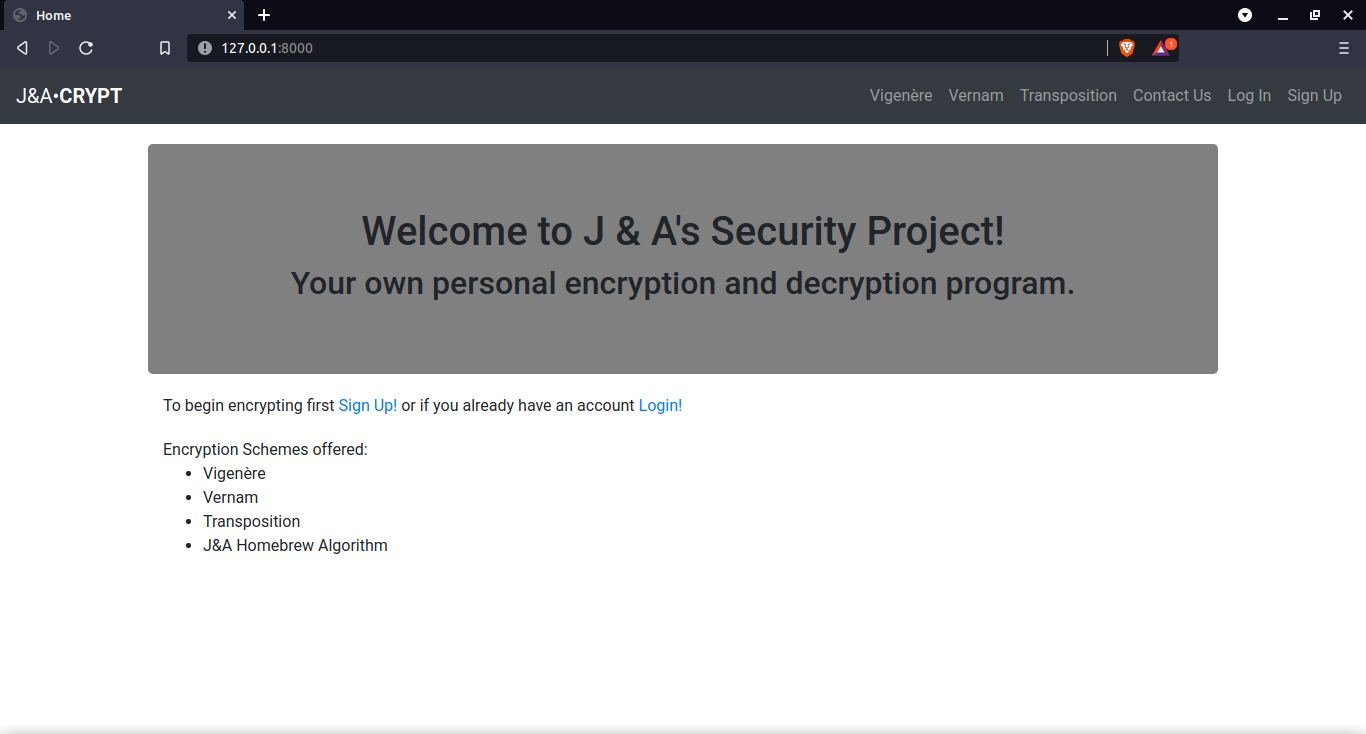
\includegraphics[scale=0.35]{./pics/index}
\caption{Our Homepage}
\end{figure}
\section{Login and Signup}
To use the features of our site you have to create an account. This can be done by clicking on the Sign Up button on the navigation bar or by going to the link:\\ \url{http://127.0.0.1:8000/accounts/signup/}\\
Some key features of our program include the process of password strength testing. This means if your password is weak you will receive feedback telling you to change it.
\begin{figure}[H]
\centering
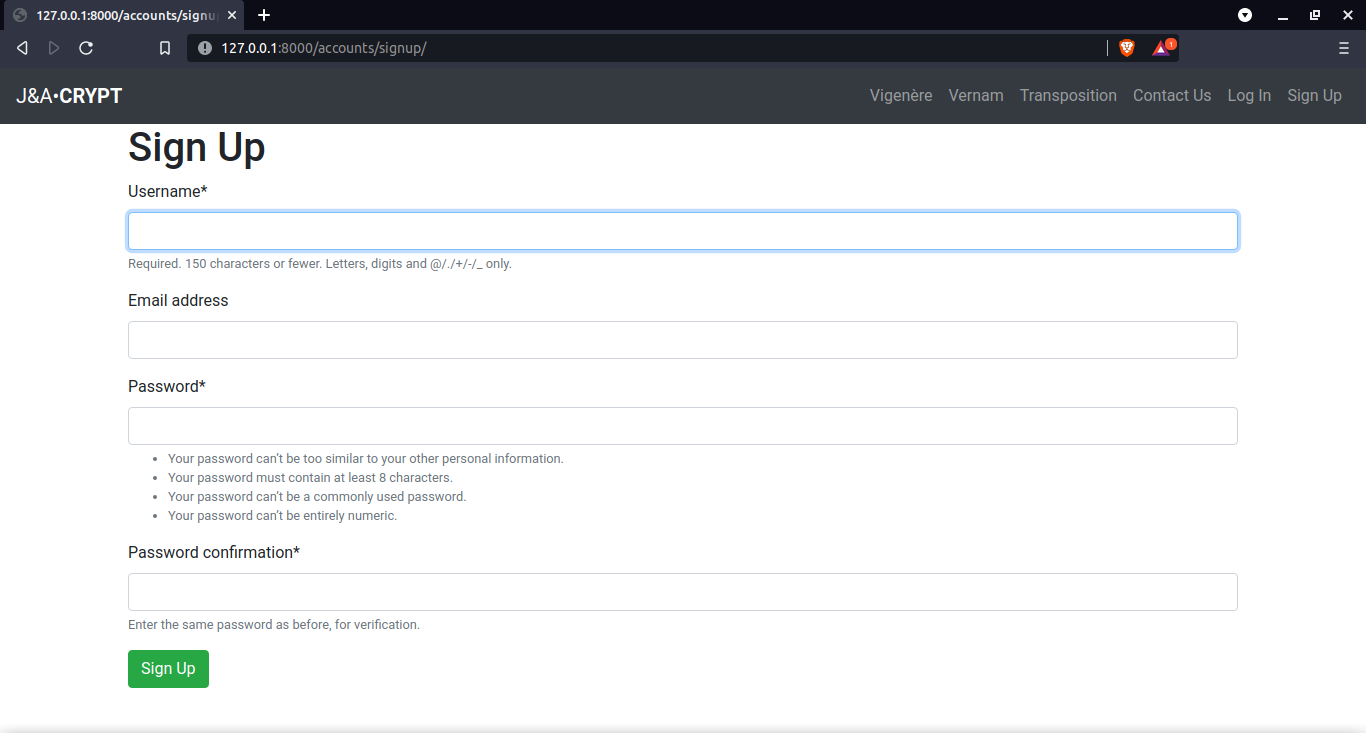
\includegraphics[scale=0.3]{./pics/signup}
\caption{Our Sign Up page}
\end{figure}
\noindent If you are already a registered user you will be able to login. This can be done by clicking on the Log In button or going to the link:\\
\url{http://127.0.0.1:8000/accounts/login/}
\begin{figure}[H]
\centering
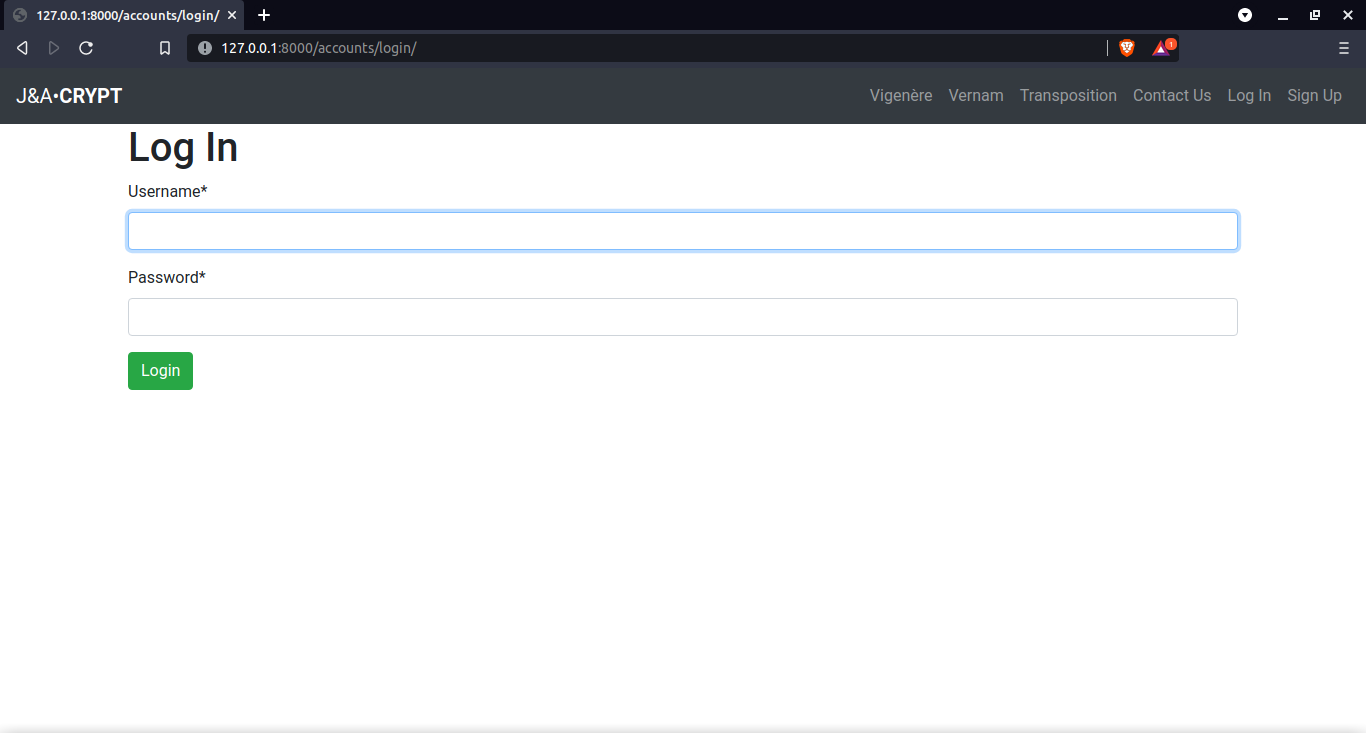
\includegraphics[scale=0.3]{./pics/login}
\caption{Our Log In page}
\end{figure}
\section{Text Encryption \& Decryption}
Once you are logged in you will be able to use the different facilities offered by our program. Our program offers Encryption \& Decryption of Text by using 4 different cryptographic schemes i.e. \texttt{Vernam}, \texttt{Vigenere}, \texttt{Transposition}, and our own \texttt{J\&A Homebrew}.\\
To Encrypt text follow the following steps:
\begin{enumerate}
\item Click on drop-down list with the scheme you want to utilise.
\item Select \textbf{Text Encryption} or \textbf{Text Decryption}.
\item Fill in the form that pops us.
\item Click on \textbf{Encrypt} or \textbf{Decrypt}
\end{enumerate}
Below is an example Screenshot of a Vigenere Text Encryption and Decryption Form.
\begin{figure}[H]
\centering
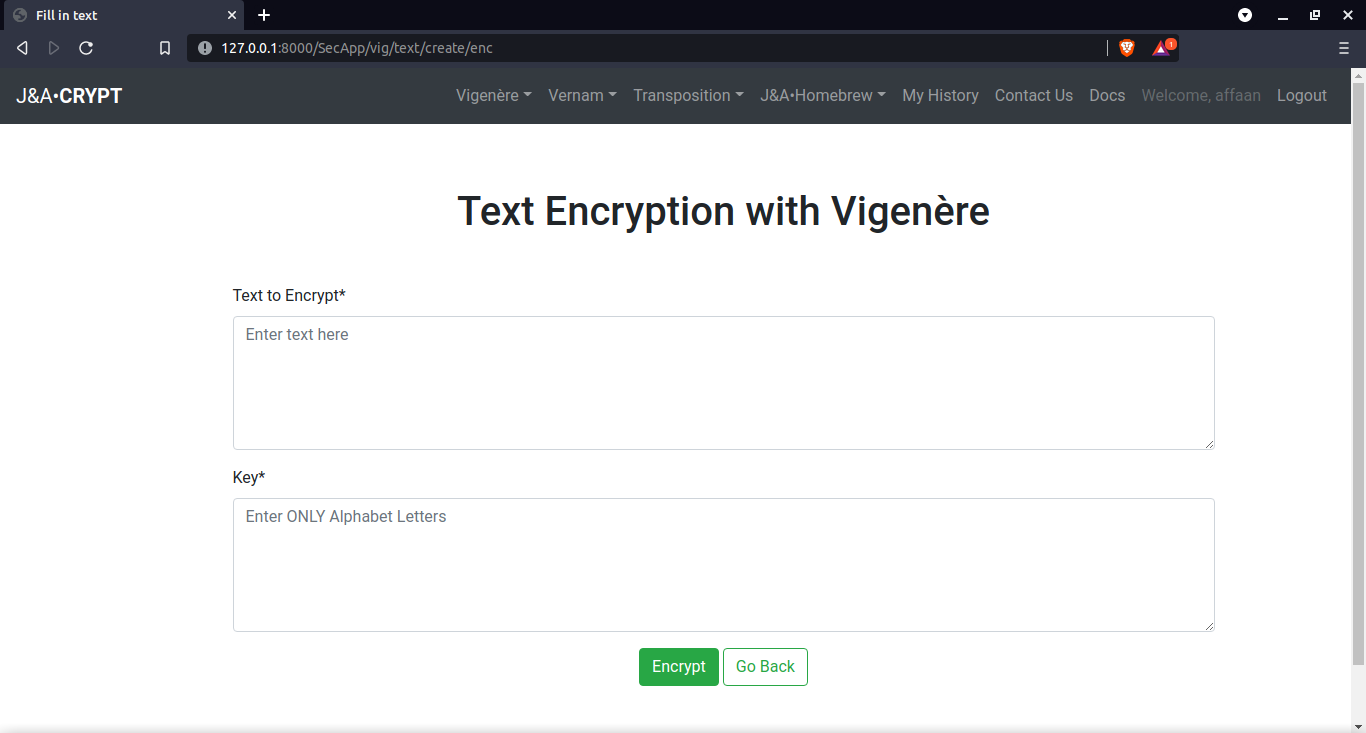
\includegraphics[scale=0.3]{./pics/vigtextenc}
\caption{Example of our Vigenere Text Encryption form}
\end{figure}
\begin{figure}[H]
\centering
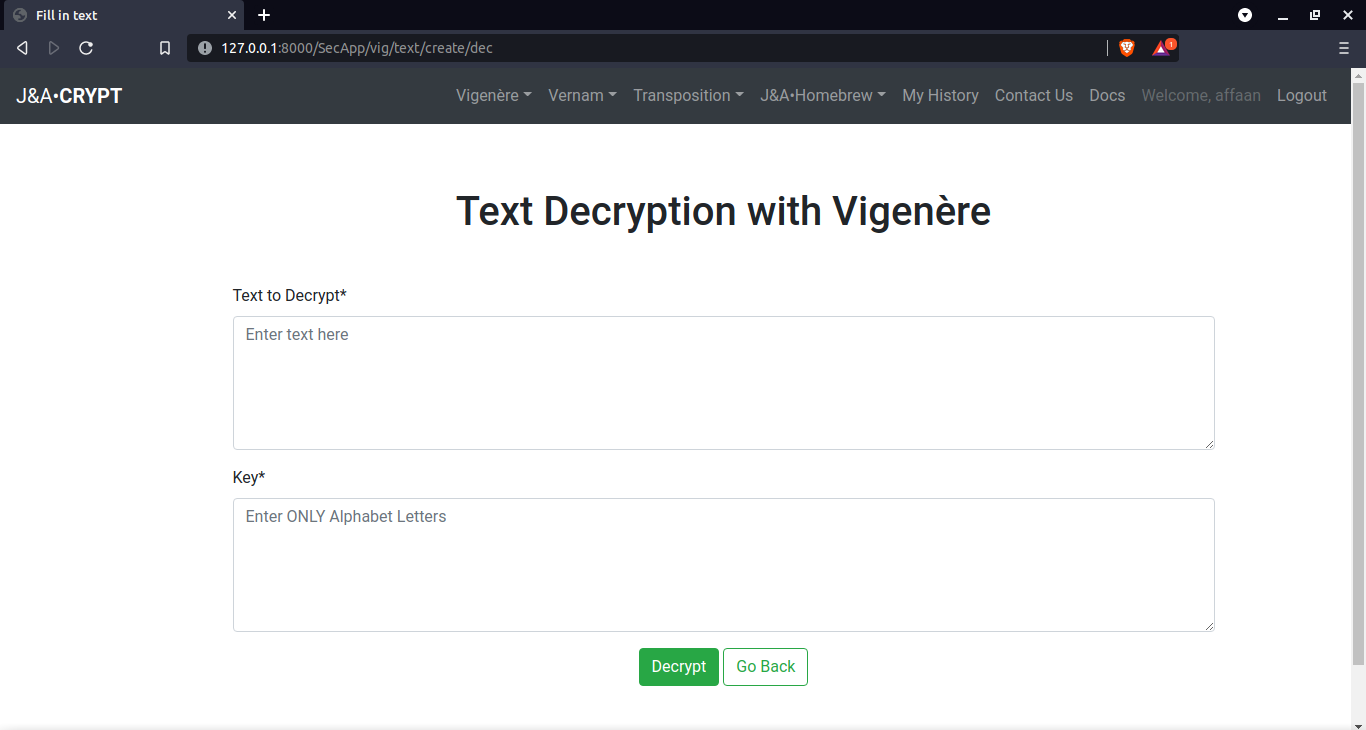
\includegraphics[scale=0.3]{./pics/vigtextdec}
\caption{Example of our Vigenere Text Decryption form}
\end{figure}
\section{File Encryption \& Decryption}
Once you are logged in you will be able to use the different facilities offered by our program. Our program offers Encryption \& Decryption of Files by using 4 different cryptographic schemes i.e. \texttt{Vernam}, \texttt{Vigenere}, \texttt{Transposition}, and our own \texttt{J\&A Homebrew}.\\
To Encrypt or Decrypt Files follow the following steps:
\begin{enumerate}
\item Click on drop-down list with the scheme you want to utilise.
\item Select \textbf{File Encryption} or \textbf{File Decryption}.
\item Fill in the form that pops us.
\item Click on \textbf{Encrypt} or \textbf{Decrypt}
\end{enumerate}
Below is an example Screenshot of a Vigenere File Encryption and Decryption Form.
\begin{figure}[H]
\centering
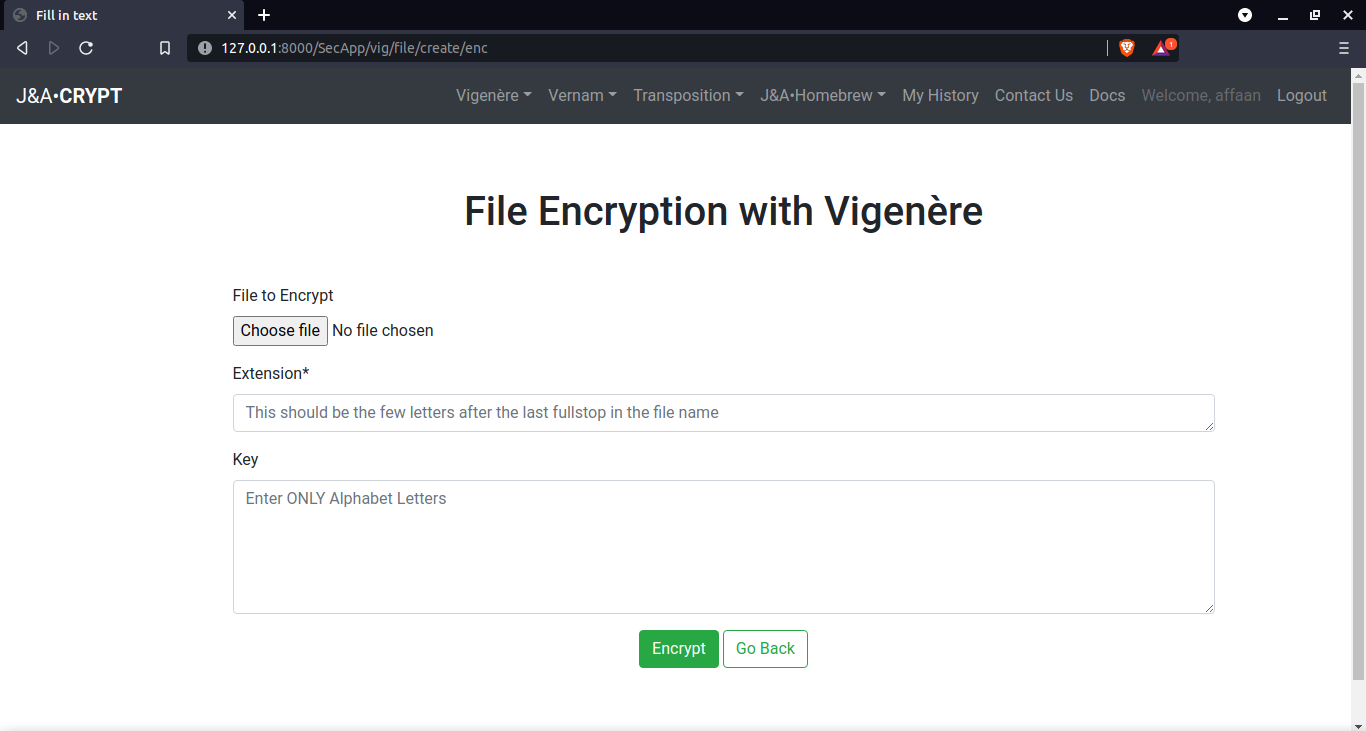
\includegraphics[scale=0.3]{./pics/vigfileenc}
\caption{Example of our Vigenere Text Encryption form}
\end{figure}
\begin{figure}[H]
\centering
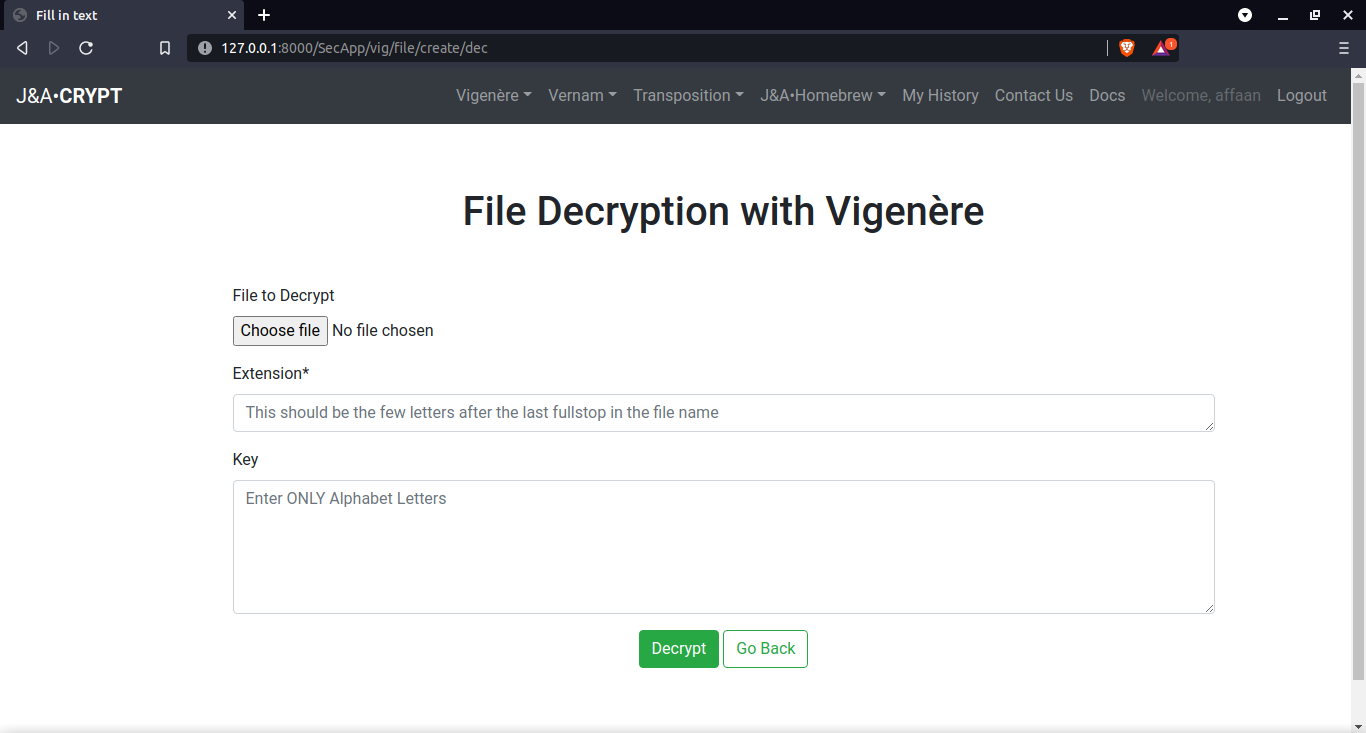
\includegraphics[scale=0.3]{./pics/vigfiledec}
\caption{Example of our Vigenere File Decryption form}
\end{figure}
\section{Documentation and Contact}
Our documentation can be found at \url{http://127.0.0.1:8000/docs/} or by clicking on the Docs button on the navigation bar.
\begin{figure}[H]
\centering
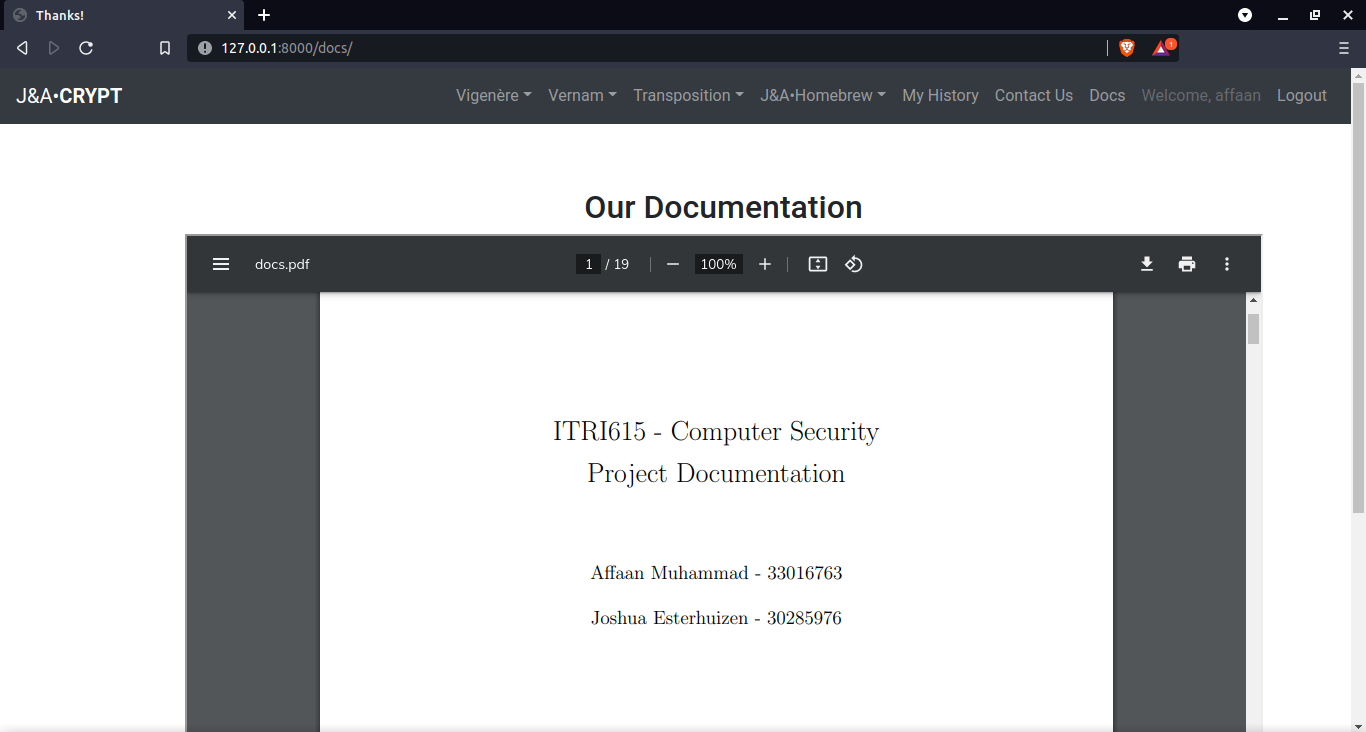
\includegraphics[scale=0.3]{./pics/docs}
\caption{Our Documentation page}
\end{figure}
Our contact details can be found at \url{http://127.0.0.1:8000/contact/} or by clicking on the Contact Us button on the navigation bar.
\begin{figure}[H]
\centering
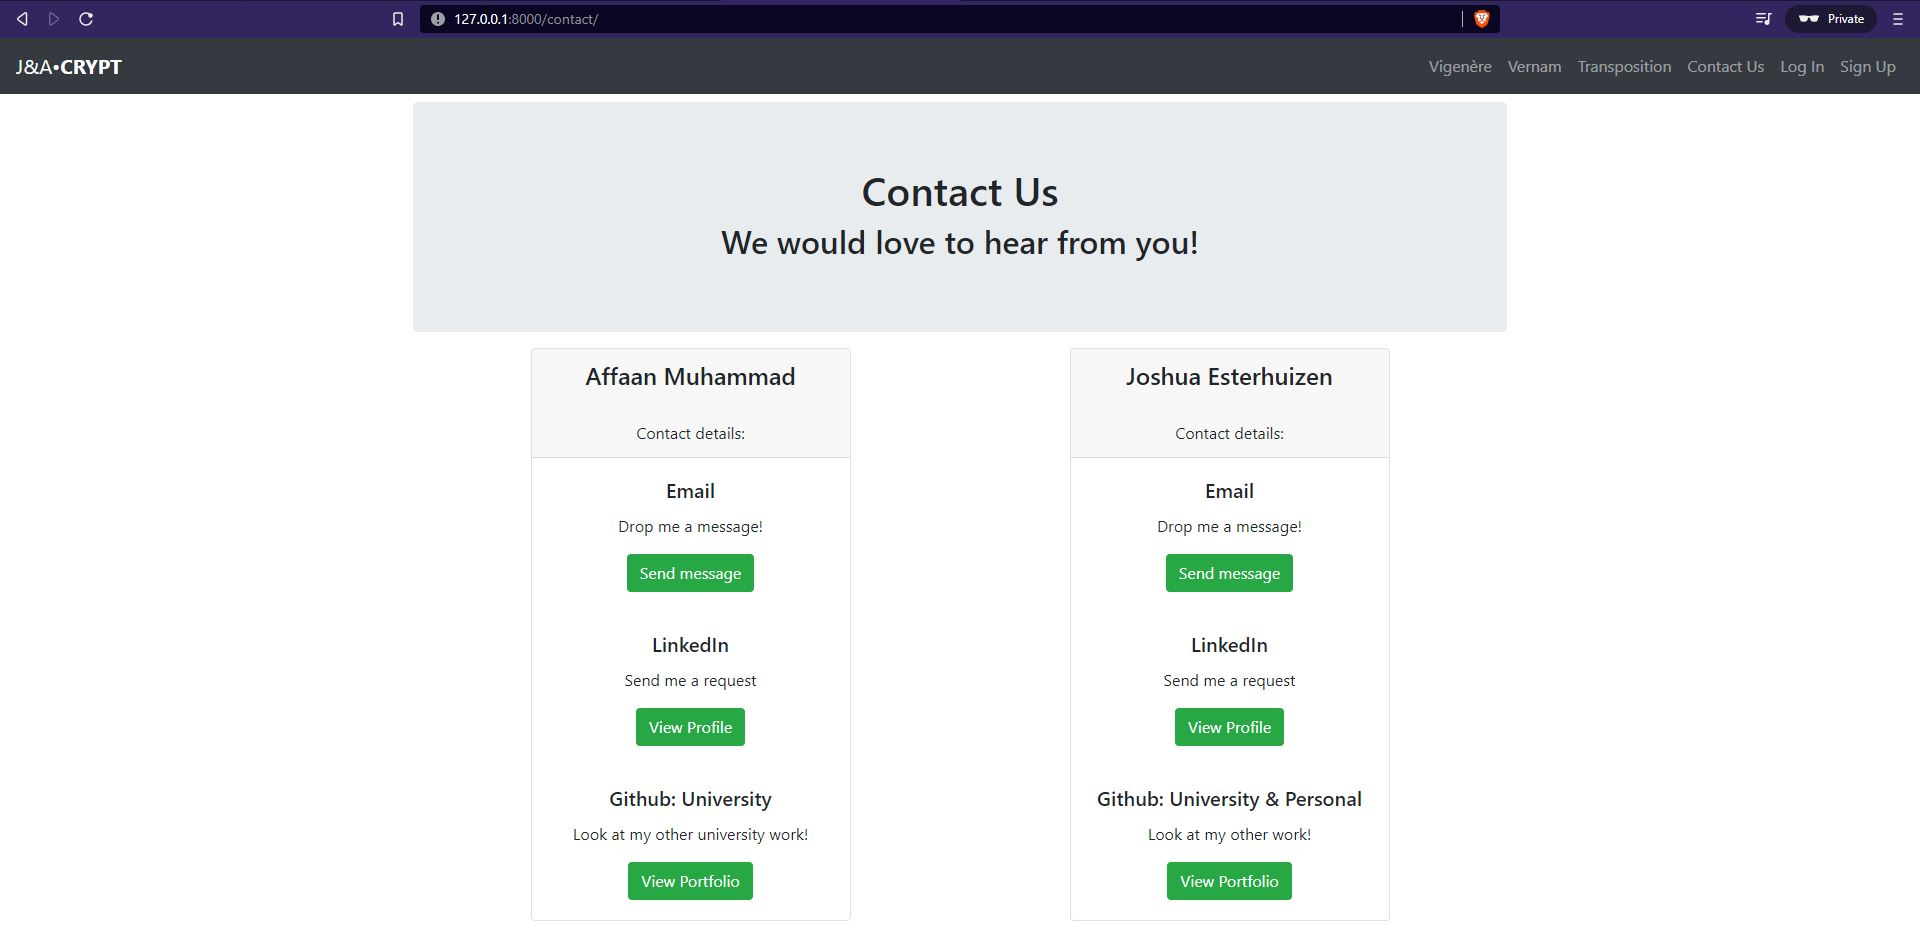
\includegraphics[scale=0.3]{./pics/contact}
\caption{Our Contact Us page}
\end{figure}
\chapter{Closing remarks}
\section{Reflection}
Joshua Esterhuizen had the following to say:
\begin{displayquote}
While developing the Vigenère and Vernam algorithms, it was very interesting how similar they are to each other in their encryption and decryption methods digitally as, through our implementation, both made use of the ASCII values of characters.
\\
While Python has great success when handling text-based files (.txt, .csv, etc.) it was not as effective when it came to other formats such as .png and .mp3 and as such imposed certain restrictions on how our algorithms could function - the most notable being that we could not alter the data type of the contents of a file to anything other than in integer byte value as it would seem that the encoding used on these is not one of the common ones like UTF-8 or UTF-32 and as such forced us to implement two "modes" for each algorithm - one for text and one for any file (.txt included)
\\
There was also an instance when testing the Vernam cipher against a .png file where the encrypted file was actually not "corrupted" (as all bytes in a file are used this included file-type specifications) and appeared as an image of a few white stripes (nothing like the original). This is interesting as the OTP generated in that instance must have had a sequence that allowed the file-type specification to still be readable and as such the file could be opened. This does pose an interesting question that if a key could be generated with certain values, could the encrypted file or text mirror the original due to the modulo calculations? While our Vernam implementation shouldn't lead to this as the OTP is diffused within the encrypted contents - it could happen with the Vigenère Cipher as the user must stipulate the key both times and it is not stored. It is very very highly unlikely to happen on file encryption due to the sheer amount of data that this would need to happen to, but for the text encryption, it could (although still very unlikely).
\end{displayquote}
\pagebreak
Affaan Muhammad had the following to say:
\begin{displayquote}
Communication was key to collaboration and the success of our project. It gives a good indication of how things will be in the industry where team development is a norm. The communication channel had to remain open and honest throughout the entire process as problems couldn't be fixed on either the backend or the frontend if the understanding was not there. For security to be successful you have to have decent documentation as well as guidance for a user. Therefore we used that in mind to help make it easy for a user to use our program and also receive feedback on what they are doing.
File Management seemed to be a bit tricky throughout the development process. Luckily we put our heads together and overcame the issues.
Learning to use CI/CD techniques definitely helped us collaborate more easily and keep our work up to date.
\end{displayquote}
\section{Work Consensus}
Below is a table showing how the work was divided in this project amongst the 2 members.
\begin{table}[H]
\centering
\begin{tabular}{@{}ll@{}}
\toprule
\multicolumn{1}{c}{Affaan}   & \multicolumn{1}{c}{Joshua}         \\ \midrule
Graphical User Interface     & Algorithms for ciphers             \\
\texttt{Models}, \texttt{Views}, and \texttt{Templates} & File and Text Management methods            \\
Testing                      & Testing                            \\
Bug fixes                    & Bug fixes                          \\
Video                        & Video                              \\
Documentation                & Overview and Background of ciphers \\ \bottomrule
\end{tabular}
\end{table}
\chapter{Sources and Acknowledgements}
\url{https://conda.io/projects/conda/en/latest/user-guide/tasks/manage-environments.html}\\
\url{https://www.udemy.com/course/python-and-django-full-stack-web-developer-bootcamp/}\\
\url{https://docs.djangoproject.com/en/3.2/}\\
\url{https://docs.python.org/3/library/math.html}\\
\url{https://docs.python.org/3/library/random.html}\\
\url{https://docs.python.org/3/c-api/list.html}\\
\url{https://docs.python.org/3/tutorial/inputoutput.html}\\
\url{https://youtu.be/h12g__mLboo}\\
\url{https://youtu.be/T9Fe-WD5Bvw}\\
\end{document}
